\chapter{Fractional Brownian Motion}
%\section{Fractional Brownian Motion}
This chapter is based on \cite{fBMbook} unless specified otherwise.

In this section, we assume that every random variable $X_{t}$ is defined on some appropriate probability space $(\Omega, \mathcal{F},\mathbb{P})$. Furthermore, we assume that the index set $I$ is either equal to $\R$, $[0,\infty)$ or $[0,T]$ for some $T>0$. 
\begin{defn}[\textit{Gaussian Process}]
    A stochastic process $X=(X_{t})_{t\in I}$ is said to be Gaussian if for all $d\geq 1$ and all $t_{1},\dots,t_{d}\in I$, $(X_{t_{1}},\dots,X_{t_{d}})$ is a Gaussian random vector. The mean function $m: I\to \R$ of $X$ is given by $m(t)=\mathbb{E}[X_{t}]$, and the covariance function $\gamma: I^{2}\to\R$ of $X$ is given by $\gamma(s,t)=\textrm{Cov}(X_{s},X_{t})$. If $m\equiv 0$, $X $ is said to be centered.
\end{defn}

\begin{defn}[\textit{Positive Semidefinite Function}]
    A symmetric function $\gamma: I^{2}\to \R$ is said to be positive semidefinite if
    \begin{equation}\label{posdef}
        \sum_{i=1}^{d}\sum_{j=1}^{d}a_{i}a_{j}\gamma(t_{i},t_{j})\geq 0
    \end{equation}
    for all $d\geq 1$, $t_{1},\dots,t_{d}\in I$, and $a_{1},\dots,a_{d}\in\R$.
\end{defn}
In fact, the condition \eqref{posdef} is equivalent to the matrix $\Gamma=\big\{\gamma (t_{i},t_{j})\big\}_{i,j=1}^{d}$ being a positive semidefinite matrix for all $d\geq 1$ and $t_{1},\dots,t_{d}\in I$.

\begin{thm}[\textit{Kolmogorov}]\label{kolmogorov}
    Let $\gamma: I^{2}\to\R$ be a symmetric function. Then there exists a centered Gaussian process $X=(X_{t})_{t\in I}$ having $\gamma$ for covariance function, if and only if $\gamma$ is positive semidefinite.
\end{thm}
\begin{lem}[\textit{Kolmogorov-Centsov}]
    Let $I=[0,T]\subset [0,\infty)$ be a compact interval for $T>0$, and let $X=(X_{t})_{t\in I}$ be a centered Gaussian process. Suppose there exists $C,\eta>0$ such that for all $s,t\in I$
    \begin{equation}
        \mathbb{E}\left[(X_{t}-X_{s})^{2}\right]\leq C|t-s|^{\eta}.
    \end{equation}
    Then, for all $\alpha\in (0,\eta/2)$, there exists a continuous modification $Y$ of $X$ with $\alpha$-Hölder continuous path. In particular, $X$ admits a continuous modification.
\end{lem}
The $\alpha$-Hölder continuity of the paths of $Y$ means there exists $C_{\alpha}\geq 0$ such that
\begin{equation}
    |Y_{t}(\omega)-Y_{s}(\omega)|\leq C_{\alpha}|t-s|^{\alpha},\quad \forall s,t\in I,\hspace{2 pt}\forall\omega\in\Omega\setminus N,
\end{equation}
where $N$ is a $\mathbb{P}$-zero set.
\begin{thm}\label{existencethm}
  Let $H>0$ be a real parameter. Then there exists a continuous centered Gaussian process $B^{H}=(B_{t}^{H})_{t\geq 0}$ with covariance function
  \begin{equation}
      \gamma_{H}(t,s)=\frac{1}{2}(t^{2H}+s^{2H}-|t-s|^{2H}), \quad s,t\geq 0,
  \end{equation}
  if and only if $H\leq 1$. In this case, the paths of $B^{H}$ are $\alpha$-Hölder continuous on each compact set $I\subset [0,\infty)$ for any $\alpha\in (0,H)$.
\end{thm}
%\begin{proof}
%    According to the Kolmogorov Theorem \ref{kolmogorov}, to show the existence of $B^{H}$, we have to show that $\gamma_{H}$ is positive semidefinite if and only $H\leq 1$.
%    Assume first that $H>1$, and take $t_{1}=1$, $t_{2}=2$, $a_{1}=-2$, and $a_{2}=1$. Then consider
%    \begin{align}
%        a_{1}^{2}\gamma_{H}(t_{1},t_{1})+2a_{1}a_{2}\gamma_{H}(t_{1},t_{2})+a_{2}^{2}\gamma_{H}(t_{2},t_{2})=4-2^{2H}<0.
%    \end{align}
%    Thus, $\gamma_{H}$ is not positive semidefinite when $H>1$. If $H=1$, then $\gamma_{1}(s,t)=st$ is indeed positive semidefinite such that for all $d\geq 1$, $t_{1},\dots,t_{d}\geq 0$, and $a_{1},\dots,a_{d}\in \R$
%    \begin{equation}
        %\sum_{i=1}^{d}\sum_{j=1}^{d}a_{i}a_{j}\gamma_{1}(t_{i},t_{j})= \left(\sum_{i=1}^{d}t_{i}a_{i}\right)^{2}\geq 0.
    %\end{equation}
    %Suppose $H\in (0,1)$
%\end{proof}
The proof of Theorem \ref{existencethm} is omitted. We will now define a fractional Brownian motion as the process, which existence is given by Theorem \ref{existencethm}.
\begin{defn}[\textit{Fractional Brownian Motion}]
    Let $H\in (0,1]$. A fractional Brownian motion (fBM) of Hurst index $H$ is a continuous centered Gaussian process $B^{H}=(B_{t}^{H})_{t\geq 0}$ such that $B_{0}^{H}=0$ almost surely and with covariance function
    \begin{equation}
        \gamma_{H}(t,s)=\mathbb{E}[B_{t}^{H}B_{s}^{H}]=\frac{1}{2}\left(t^{2H}+s^{2H}-|t-s|^{2H}\right).
    \end{equation}
\end{defn}
Proposition \ref{prop211} and \ref{prop212} exhibit some properties of the fractional Brownian motion.
\begin{prop}\label{prop211}
    Let $B^{H}$ be a fractional Brownian motion of Hurst index $H\in (0,1]$.
    \begin{enumerate}
        \item If $H=1/2$, then $B^{H}$ is just a standard Brownian motion.
        \item If $H=1$, then $B^{H}_{t}=tB_{1}^{H}$ almost surely for all $t\geq 0$.
    \end{enumerate}
\end{prop}
\begin{proof}
    For $H=1/2$, we immediately see that
    \begin{align}
        \mathbb{E}[B_{t}^{1/2}B_{s}^{1/2}]&=\frac{1}{2}\left(t+s-|t-s|\right)\\
        &= \frac{1}{2}\left(t+s-2 \min\{s,t\}-s-t\right)\\
        &= s\land t,
    \end{align}
    so $B^{1/2}$ is a standard Brownian motion.

    Let $H=1$. Then for all $t\geq 0$, we have
    \begin{align}
        \mathbb{E}\left[(B^{1}_{t}-tB_{1}^{1})^{2}\right]&= \mathbb{E}\left[(B_{t}^{1})^{2}\right]-2t\mathbb{E}\left[B_{t}^{1}B_{1}^{1}\right]+t^{2}\mathbb{E}\left[(B_{1}^{1})^{2}\right]\\
        &= t^{2}-t\left(t^{2}+1-(1-t)^{2}\right)+t^{2}\\
        &= 0,
    \end{align}
    so $B_{t}^{1}=tB_{1}^{1}$ almost surely.
\end{proof}
In particular, Proposition \ref{prop211} shows that it suffices to only consider fractional Brownian motions with Hurst index $H\in (0,1)$.
 \begin{prop}\label{prop212}
     Let $B^{H}$ be a fractional Brownian motion of Hurst index $H\in (0,1)$. Then we have
     \begin{enumerate}
         \item (Self-similarity) For all $a>0$, $\left(a^{-H}B^{H}_{at}\right)_{t\geq 0}\mylaw(B_{t}^{H})_{t\geq 0}$.
         \item (Stationarity of Increments) For all $h>0$, $\left(B_{t+h}^{H}-B_{h}^{H}\right)_{t\geq 0}\mylaw (B_{t}^{H})_{t\geq 0}$.
         \item (Time Inversion) $\left(t^{2H}B^{H}_{1/t}\right)_{t>0}\mylaw (B_{t}^{H})_{t>0}$.
     \end{enumerate}
     Conversely, any continuous Gaussian process $B^{H}=(B_{t}^{H})_{t\geq 0}$ with $B_{0}^{H}=0$, $\textrm{Var}[B_{1}^{H}]=1$, and such that 1. and 2. above hold, is a fractional Brownian motion of Hurst index $H$.
 \end{prop}
 \begin{proof}
 To prove self-similarity, we see that
     \begin{align}
         \mathbb{E}\left[a^{-H}B_{at}^{H}a^{-H}B_{as}^{H}\right]&=a^{-2H}\mathbb{E}[B_{at}^{H}B_{as}^{H}]\\
         &=\frac{a^{-2H}}{2}\left((at)^{2H}+(as)^{2H}-|at-as|^{2H}\right)\\
         &= \frac{1}{2}(t^{2H}+s^{2H}-|t-s|^{2H}).
     \end{align}
     The proof of 2. and 3. are completely analogous, and are therefore omitted. Conversely, let $B^{H}=(B_{t}^{H})_{t\geq 0}$ be a continuous Gaussian process with $B^{H}_{0}=0$ and $\textrm{Var}[B_{1}^{H}]=1$, which additionally satisfies 1. and 2. Using 2. with $t=h>0$, we get $\mathbb{E}[B_{2t}^{H}]=2\mathbb{E}[B_{t}^{H}]$, and using 1. we infer that $\mathbb{E}[B_{2t}^{H}]=2^{H}\mathbb{E}[B_{t}^{H}]$. Combining these two equalities gives $\mathbb{E}[B_{t}^{H}]=0$ for all $t>0$, and thus $B^{H}$ is centered. Let $s,t\geq 0$. Then we infer that
     \begin{align}
         \E[B_{s}^{H}B_{t}^{H}]&=\frac{1}{2}\left(\E\left[(B_{t}^{H})^{2}\right]+\E\left[(B_{s}^{H})^{2}\right]-\E\left[(B_{t}^{H}-B_{s}^{H})^{2}\right]\right)\\
         &= \frac{1}{2}\left(\E\left[(B_{t}^{H})^{2}\right]+\E\left[(B_{s}^{H})^{2}\right]-\E[(B_{|t-s|}^{H})^{2}]\right)\\
         &= \frac{1}{2}\E[(B_{1}^{H})^{2}]\left(t^{2H}+s^{2H}-|t-s|^{2H}\right)\\
         &= \frac{1}{2}\left(t^{2H}+s^{2H}-|t-s|^{2H}\right),
     \end{align}
     which concludes the proof.
 \end{proof}
\begin{defn}[\textit{Fractional Gaussian Noise}]
    Let $B^{H}= (B_{t}^{H})_{t\geq 0}$ be a fractional Gaussian process of Hurst index $H\in (0,1)$. Then the increments defined as
    \begin{equation}
        \Delta B_{t}^{H}\coloneqq B_{t+h}^{H}-B_{t}^{H}, \quad h>0,
    \end{equation}
    are called fractional Gaussian noise.
\end{defn}
We have the following proposition.
\begin{prop}\label{corr}
    Let $B^{H}=(B_{t}^{H})_{t\geq 0}$ be a fractional Brownian motion of Hurst index $H\in (0,1)$. Then disjoint increments of $B^H$ are negatively correlated for $H\in (0,1/2)$, positively correlated for $H\in (1/2,1)$, and uncorrelated for $H=1/2$.
\end{prop}
\begin{proof}
Let $\Delta B_{t}^{H}=B_{t+h}^{H}-B_{t}^{H}$ and $\Delta B_{s}^{H}=B_{s+h}^{H}-B_{s}^{H}$ be increments of a fractional Brownian motion $B^{H}$ such that $s+h< t$ and $t-s=nh$, $n\in \N$ so as to ensure $[s,s+h]\cap [t,t+h]=\emptyset$. Then the covariance of the increments is given as
\begin{align*}
    \E\left[\Delta B_{t}^{H}\Delta B_{s}^{H}\right]&=\E[B_{t+h}^{H}B_{s+h}^{H}]-\E[B_{t+h}^{H}B_{s}^{H}]-\E[B_{t}^{H}B_{s+h}^{H}]+\E[B_{t}^{H}B_{s}^{H}]\\
    &= \frac{1}{2}\left((t+h)^{2H}+(s+h)^{2H}-|nh|^{2H}\right)-\frac{1}{2}\left((t+h)^{2H}+s^{2H}-|h(n+1)|^{2H}\right)\\
    & -\frac{1}{2}\left(t^{2H}+(s+h)^{2H}-|h(n-1)|^{2H}\right)+ \frac{1}{2}\left(t^{2H}+s^{2H}-|nh|^{2H}\right)\\
    &=  \frac{1}{2}h^{2H}\left((n+1)^{2H}+(n-1)^{2H}-2n^{2H}\right).
\end{align*}
Thus, for a fixed $h$, the covariance of the increments only depends on $n\in \N$. Define the function $f:[1,\infty)\to \R$ by
\begin{equation}
f(x)\coloneqq (x+1)^{2H}+(x-1)^{2H}-2x^{2H}.
\end{equation}
Then, it is easy to see that $f(x)>0$, $\forall x\in [1,\infty)$ if $H>1/2$, and $f(x)<0$, $\forall x\in [1,\infty)$ if $H<1/2$. In the case of $H=1/2$, the increments are independent, and by virtue of the Brownian motion being a Gaussian process, they are consequently also uncorrelated.
    %Suppose that $0\leq s_{1}<t_{1}<s_{2}<t_{2}$ such that $[s_{1},t_
    %{1}]\cap [s_{2},t_{2}]=\emptyset$. Then the covariance of the increments is given as
    %\begin{align*}
        %\E\left[(B_{t_{1}}^{H}-B_{s_{1}}^{H})(B_{t_{2}}^{H}-B_{s_{2}}^{H})\right] &= \E[B_{t_{1}}^{H}B_{t_{2}}^{H}]-\E[B_{t_{2}}^{H}B_{s_{1}}^{H}]-\E[B_{t_{1}}^{H}B_{s_{2}}^{H}] + \E[B_{s_{1}}^{H}B_{s_{2}}^{H}]\\
        %&= \frac{1}{2}\left(|t_{2}-s_{1}|^{2H}-|t_{2}-t_{1}|^{2H}-\left(|s_{2}-s_{1}|^{2H}-|s_{2}-t_{2}|^{2H}\right)\right).
    %\end{align*}
    %Now, define the function $f(x)=|x|^{2H}$ and put $a_{1}\coloneqq t_{2}-s_{1}$, $a_{2}\coloneqq t_{2}-t_{1}$, $b_{1}\coloneqq s_{2}-s_{1}$, and $b_{2}\coloneqq s_{2}-t_{2}$. Note that $b_{2}<a_{2}<b_{1}<a_{1}$. This allows the covariance of the increments to be expressed as 
    %\begin{equation}
        %\E\left[(B_{t_{1}}^{H}-B_{s_{1}}^{H})(B_{t_{2}}^{H}-B_{s_{2}}^{H})\right]=\frac{1}{2}\left(f(a_{1})-f(a_{2})-\left(f(b_{1})-f(b_{2})\right)\right).
    %\end{equation}
\end{proof}
A consequence of Proposition \ref{corr} is that the increments $X_{k}\coloneqq B_{k}^{H}-B_{k-1}^{H}$ and $X_{k+n}\coloneqq B_{k+n}^{H}-B_{k+n-1}^{H}$ of a fBM $B^{H}$ exhibit long memory for $H>1/2$, since the auto-covariance function satisfies
\begin{equation}\label{asymp}
\gamma_{H}(n)\coloneqq \frac{1}{2}\left((n+1)^{2H}+(n-1)^{2H}-2n^{2H}\right) \sim H(2H-1)n^{2H-2},
\end{equation}
as $n\to\infty$. Here $f(n)\sim g(n)$ is used to indicate that $\lim_{n\to\infty}f(n)/g(n)=1$. Thus, we obtain that $\sum_{n=1}^{\infty}|\gamma_{H}(n)|=\infty$ for $H>1/2$ and $\sum_{n=1}^{\infty}|\gamma_{H}(n)|<\infty$ for $H<1/2$. Hence, a fBM can be used to model both long and short memory, when the Hurst index is chosen appropriately. 
%It is well-known that a discrete weakly stationary stochatic process $(X_{n})_{n\in \N}$ is said to exhibit long memory if its autocovariance function $\rho(n)\coloneqq \textrm{Cov}(X_{k},X_{k+n})$ satisfies $\rho(n)\sim Kn^{2d-1}$, i.e.
%\begin{equation}
%    \lim_{n\to \infty}\frac{\rho(n)}{Kn^{2d-1}}=1,
%\end{equation}
%for some non-zero constant $K$ and $d \in (0,1/2)$. In this case, we have that $\sum_{n=1}^{\infty}\rho(n)=\infty$. Consequently, we obtain that the increments $X_{k}\coloneqq B^{H}_{k}-B^{H}_{k-1}$ and $X_{k+n}\coloneqq B^{H}_{k+n}-B^{H}_{k+n-1}$ of a fBM $B^H$ exhibit long memory for $H>1/2$, since 
%\begin{equation}\label{asymp}
%    \rho_{H}(n)\coloneqq \frac{1}{2}\left((n+1)^{2H}+(n-1)^{2H}-2n^{2H}\right) \sim H(2H-1)n^{2H-2},
%\end{equation}
%as $n\to \infty$. Thus, we obtain that $\sum_{n=1}^{\infty}|\rho_{H}(n)|=\infty$ for $H>1/2$, and $\sum_{n=1}^{\infty}|\rho_{H}(n)|<\infty$ for $H<1/2$.
\section{Non-Semimartingale Property}
In this section, we will study the asymptotic properties of the $p$-variations of a fBM. Additionally, we will show that a fBM is not a semimartingale except for when $H=1/2$. Firstly, we introduce the class of Hermite polynomials and a useful lemma.
\begin{defn}[\textit{Hermite Polynomials}]
    The Hermite polynomials are defined as the family $(H_{k})_{k\in \N}\subset \R[x]$ of polynomials satisfying
    \begin{equation}
        H_{k}(x)=(\delta^{k}1)(x), \quad k\in\N,
    \end{equation}
    where $1$ is the function constantly equal to $1$, and $(\delta\varphi)(x)\coloneqq x\varphi(x)-\varphi'(x)$ for $\varphi\in C^{1}$.
\end{defn}
\begin{lem}\label{l2lemma}
    Let $(h_{k})_{k\in \N}$ be the family of Hermite polynomials. Then $(\frac{1}{\sqrt{k!}}H_{k})_{k\in\N}$ is an orthonormal basis of $L^{2}\left(\R,\mathcal{B}(\R),\nu\right)$, where $\nu$ is the standard Gaussian measure
    \begin{equation}
        \nu(A)\coloneqq \frac{1}{\sqrt{2\pi}}\int_{A}e^{-x^{2}/2}dx,\quad A\in\mathcal{B}(\R).
    \end{equation}
\end{lem}
We present the following theorem, which may be viewed as a law of large numbers for fractional Brownian motions.
\begin{thm}\label{llnthm}
    Let $G\sim\mathcal{N}(0,1)$ and let $f:\R\to\R$ be a measurable function such that $\E[f^{2}(G)]<\infty$. Let $B^H$ be a fractional Brownian motion of Hurst index $H\in (0,1)$. Then, as $n\to\infty$
    \begin{equation}\label{lln}
        \frac{1}{n}\sum_{i=1}^{n}f(B^{H}_{i}-B^{H}_{i-1})\overset{L^{2}}{\to} \E[f(G)]
    \end{equation}
\end{thm}
Note that using the self-similariy property, we can rewrite \eqref{lln} as
\begin{equation}
     \frac{1}{n}\sum_{i=1}^{n}f\left(n^{H}(B^{H}_{i/n}-B^{H}_{(i-1)/n})\right)\overset{L^{2}}{\to} \E[f(G)] \hspace{6 pt}\mathrm{as}\hspace{5 pt}n\to\infty.
\end{equation}
\begin{proof}
    If $H=1/2$, then the result follows from the classical law of large numbers, since the increments then $B^{1/2}_{i}-B^{1/2}_{i-1}\overset{\textrm{i.i.d}}{\sim} \mathcal{N}(0,1)$. Assume now that $H\neq 1/2$. Since $\E[f^{2}(G)]<\infty$, we have that $f\in L^{2}\left(\R,\mathcal{B}(\R),\nu\right)$, and as a consequence of Lemma \ref{l2lemma}
    \begin{equation}\label{infsum}
        f(x)=\sum_{k=0}^{\infty}\frac{c_{k}}{\sqrt{k!}}H_{k}(x), \quad x\in \R,
    \end{equation}
    where $H_{0}(x)\equiv 1$. By the orthogonality of the Hermite polynomials, we have $\sum_{k=0}^{\infty}c_{k}^{2}=\E[f^{2}(G)]<\infty$. Choosing $x=G$ and taking the expectation in $\eqref{infsum}$, we obtain that $c_{0}=\E[f(G)]$. Hence
    \begin{align}
        \frac{1}{n}\sum_{i=1}^{n}f(B_{i}^{H}-B_{i-1}^{H}) - \E[f(G)]&=\frac{1}{n}\sum_{i=1}^{n}\left(f(B_{i}^{H}-B_{i-1}^{H}) - \E[f(G)]\right)\\
        &= \frac{1}{n}\sum_{k=0}^{\infty}\frac{c_{k}}{\sqrt{k!}}\sum_{i=1}^{n}H_{k}(B_{i}^{H}-B_{i-1}^{H}).
    \end{align}
In the following, we will use the fact that if $(U,V)$ is a Gaussian vector with $U,V\sim\mathcal{N}(0,1)$, then for all $k,l\in\N$
\begin{equation}\label{fintresultat}
    \E[H_{k}(U)H_{l}(V)]=\begin{cases}
        k!\E[UV]^{k} & \mathrm{if}\hspace{2.5 pt} k=l,\\
        0, & \mathrm{otherwise}.
    \end{cases}
\end{equation}
Using \eqref{fintresultat}, we deduce
\begin{align}
    &\E\left[\left(\frac{1}{n}\sum_{i=1}^{n}f(B_{i}^{H}-B_{i-1}^{H}) - \E[f(G)]\right)^{2}\right]\\
    &= \frac{1}{n^2}\sum_{k=1}^{\infty}\frac{c_{k}^{2}}{k!}\sum_{i'=1}^{n}\sum_{i =1}^{n}\E[H_{k}(B^{H}_{i}-B_{i-1}^{H})H_{k}(B^{H}_{i'}-B^{H}_{i'-1})]\\
    &= \frac{1}{n^2}\sum_{k=1}^{\infty}c_{k}^{2}\sum_{i'=1}^{n}\sum_{i =1}^{n}\E[(B^{H}_{i}-B_{i-1}^{H})(B^{H}_{i'}-B^{H}_{i'-1})]^{k}\\
    &= \frac{1}{n^2}\sum_{k=1}^{\infty}c_{l}^{2}\sum_{i'=1}^{n}\sum_{i =1}^{n}\gamma_{H}(i-i')^{k},
\end{align}
where $\gamma_{H}$ is the auto-covariance function of fractional Gaussian noise
\begin{equation}
    \gamma_{H}(x)=\gamma_{H}(|x|)=\frac{1}{2}\left(|x+1|^{2H}+|x-1|^{2H}-2|x|^{2H}\right), \quad x\in \Z. 
\end{equation}
Utilizing the fact that $\gamma_{H}(x)=\E[B_{1}^{H}(B_{|x|+1}^{H}-B_{|x|}^{H})]$, and that the covariance is an inner product, we get by Cauchy-Schwarz
\begin{align}
     |\gamma_{H}(x)|\leq \sqrt{\E[(B_{1}^{H})^{2}]}\sqrt{\E[(B_{|x|+1}^{H}-B_{|x|}^{H})^{2}]}=1.
\end{align}
We are now ready to study the $L^2$-convergence of $n^{-1}\sum_{i=1}^{n}f(B_{i}^{H}-B_{i-1}^{H})-\E[f(G)]$
\begin{align}
    \E\left[\left(\frac{1}{n}\sum_{i=1}^{n}f(B_{i}^{H}-B_{i-1}^{H})-\E[f(G)]\right)^{2}\right] &\leq \frac{1}{n^{2}}\sum_{k=1}^{\infty}c_{k}^{2}\sum_{i'=1}^{n}\sum_{i =1}^{n}|\gamma_{H}(i-i')|\\
    &= \mathrm{Var}[f(G)]\frac{1}{n^2}\sum_{i'=1}^{n}\sum_{i =1}^{n}|\gamma_{H}(i-i')|\\
    &= \mathrm{Var}[f(G)]\frac{1}{n^2}\sum_{i'=1}^{n}\sum_{i=1-i'}^{n-i'}|\gamma_{H}(i)|\\
    &\leq 2\mathrm{Var}[f(G)]\frac{1}{n}\sum_{i=0}^{n-1}|\gamma_{H}(i)|.
\end{align}
We already know from \eqref{asymp} that $\gamma_{H}(i)\sim H(2H-1)i^{2H-2}$ as $i\to \infty$. We know that if $H<1/2$, then $\sum_{i=1}^{\infty}|\gamma_{H}(i)|<\infty$, and the result \eqref{lln} holds. If $H>1/2$, then $\sum_{i=1}^{n-1}|\gamma_{H}(i)|\sim H(2H-1)\sum_{i=1}^{n-1}i^{2H-2}\sim Hn^{2H-1}$ as $n\to \infty$, and the result \eqref{lln} holds as well because $H<1$.
\end{proof}
As a consequence, we have the following corollary.
\begin{cor}\label{pvariations}
    Let $B^H$ be a fractional Brownian motion of Hurst index $H\in (0,1)$, and let $p\in [1,\infty)$. Then, in $L^{2}(\Omega,\mathcal{F},\mathbb{P})$ and as $n\to\infty$, we have
    \begin{equation}
        \sum_{i=1}^{n}\left|B_{i/n}^{H}-B_{(i-1)/n}^{H}\right|^{p}\to \begin{cases}
            0, & \mathrm{if} \hspace{3 pt}p>\frac{1}{H},\\
            \E[|G|^{p}], & \mathrm{if}\hspace{3 pt}p=\frac{1}{H},\hspace{3 pt} \mathrm{with}\hspace{3 pt} G\sim \mathcal{N}(0,1),\\
            \infty, & \mathrm{if}\hspace{3 pt}p<\frac{1}{H}.
        \end{cases}
    \end{equation}
\end{cor}
\begin{proof}
    If we apply Theorem \ref{llnthm} with $f(x)=|x|^p$, we get
    \begin{align}
         \sum_{i=1}^{n}\left|B_{i/n}^{H}-B_{(i-1)/n}^{H}\right|^{p}&= \sum_{i=1}^{n}\left|n^{-H}(B_{i}^{H}-B_{i-1}^{H})\right|^{p}\\
         &= \frac{1}{n^{Hp}}\sum_{i=1}^{n}\left|B_{i}^{H}-B_{i-1}^{H}\right|^{p}\\
         &= \frac{1}{n^{H(p-1/H)}}\left(\frac{1}{n}\sum_{i=1}^{n}\left|B_{i}^{H}-B_{i-1}^{H}\right|^{p}\right)\\
         &= \frac{1}{n^{H(p-1/H)}}\E[f(G)].
    \end{align}
If $p=1/H$, then the above is simply equal to \eqref{lln}. If $p<1/H$, then $n^{-H(p-1/H)}\to \infty$ as $n\to \infty$, and conversely $n^{-H(p-1/H)}\to 0$ as $n\to \infty$ if $p>1/H$.
\end{proof}
We are now ready to prove that a fBM is not a semimartingale, except when $H=1/2$. Consequently, integration with respect to a fBM becomes a non-trivial problem, when $H\neq 1/2$.
\begin{thm}
    Let $B^H$ be a fractional Brownian motion of Hurst index $H\in (0,\frac{1}{2})\cup (\frac{1}{2},1)$. Then $B^H$ is not a semimartingale.
\end{thm}
\begin{proof}
    By selfsimilarity, it is sufficient to consider the time interval $[0,1]$ for the proof. Firstly, recall that the following two properties hold for a semimartingale $S$ on $[0,1]$
    \begin{enumerate}
        \item $\sum_{k=1}^{n}\left(S_{k/n}-S_{(k-1)/n}\right)^{2}\overset{\mathbb{P}}{\to} \langle S\rangle_{1}<\infty$ as $n\to\infty$.
        \item Moreover, if $\langle S\rangle_{1}=0$, then $S$ is of bounded variation, i.e. it holds almost surely that
        \begin{equation}
            \sup_{n\geq 1}\sum_{k=1}^{n}|S_{k/n}-S_{(k-1)/n}|<\infty. 
        \end{equation}
    \end{enumerate}
    Now, if $H<1/2$, then $\sum_{k=1}^{n}(B_{k/n}^{H}-B_{(k-1)/n}^{H})^{2}\to \infty$ by Corollary \ref{pvariations}. Hence, $B^H$ is not a semimartingale. Conversely, if $H>1/2$, then Corollary \ref{pvariations} yields $\sum_{k=1}^{n}(B_{k/n}^{H}-B_{(k-1)/n}^{H})^{2}\to 0$. Let $p\in (1,1/H)$, then Corollary \ref{pvariations} again yields $\sum_{k=1}^{n}(B_{k/n}^{H}-B_{(k-1)/n}^{H})^{p}\to \infty$. Additionally, by the uniform continuity of the paths $[0,1]\ni t\mapsto B_{t}^{H}(\omega)$, we obtain almost surely
    \begin{equation}
        \sup_{1\leq k\leq n}|B_{k/n}^{H}-B_{(k-1)/n}^{H}|^{p-1}<\varepsilon, \quad \forall \varepsilon>0.
    \end{equation}
    Combining the above, we ge the inequality
    \begin{equation}
        \sum_{k=1}^{n}\left|B_{k/n}^{H}-B_{(k-1)/n}^{H}\right|^{p}\leq \sup_{1\leq k\leq n}|B_{k/n}^{H}-B_{(k-1)/n}^{H}|^{p-1}\sum_{k=1}^{n}\left|B_{k/n}^{H}-B_{(k-1)/n}^{H}\right|
    \end{equation}
    from which we deduce that $\sum_{k=1}^{n}|B_{k/n}^{H}-B_{(k-1)/n}^{H}|\to \infty$. Consequently, $B^H$ is also not a semimartingale, when $H>1/2$.
\end{proof}
\section{Integration wrt. Fractional Brownian Motion}
In the previous section, it was shown that a fBM $B^H$ is not a semimartingale whenever $H\neq 1/2$. Consequently, the usual Itô calculus is not applicable, and alternative methods must be utilized to define and solve SDE's of the form
\begin{equation}
    X_{t}=X_{0}+\int_{0}^{t}b(s,X_{s})ds + \int_{0}^{t}\sigma(s,X_{s})dB_{s}^{H},\quad t\geq 0. 
\end{equation}
There are a variety of ways to define stochastic integration with a fractional Brownian motion as integrator, and hence there is not one unified framework for this type of stochastic calculus. Due to the non-Markovian nature of the fBM, the most natural way to define the stochastic integral is to do it pathwise for a.e. $\omega\in \Omega$. For $H>1/2$, the regularity of the paths is sufficient to define the solution pathwise using the Young integral. Our main interest is when $H<1/2$, and in this case, one possible definition is the forward integral.
\begin{defn}[\textit{Forward Integral}]\label{defn:forward}
    Let $X=(X_{t})_{t\in [0,T]}$ and $Y=(Y_{t})_{t\in [0,T]}$ be two continuous stochastic processes. Provided that the limit exists in probability, we define the forward integral of $Y$ with respect to $X$ as
    \begin{equation}
        \int_{0}^{T}Y_{s}d^{-}X_{s}=\lim_{n\to\infty}\sum_{k=0}^{n-1}Y_{kT/n}(X_{(k+1)T/n}-X_{kT/n}).
    \end{equation}
\end{defn}
Definition \ref{defn:forward} is essentially just a pathwise Riemann-Stieltjes integral. For Riemann-Stieltjes integrals, it is well-known that if $f$ is a bounded function on $[0,T]$, and $g$ is monotonically increasing on $[0,T]$ with Riemann-integrable derivative $g'$, then it holds that
\begin{equation}
    \int_{0}^{T}f(x)dg(x)=\int_{0}^{T}f(x)g'(x)dx.
\end{equation}
This intuition leads to an equivalent definition for the forward integral as
\begin{equation}\label{defn:forward2}
    \int_{0}^{T}Y_{s}d^{-}X_{s}\coloneqq \lim_{\varepsilon\to 0}\int_{0}^{T}Y_{s}\frac{X_{s+\varepsilon}-X_{s}}{\varepsilon}ds,
\end{equation}
where $X=(X_{t})_{t\in [0,T]}$ and $Y=(Y_{t})_{t\in [0,T]}$ are two continuous stochastic processes, and thus they are also Riemann-integrable. However, $X$ is not differentiable in general. Note that the left-hand side is the forward integral, and the right-hand side is just a regular Riemann-integral.  

One might ask whether this definition is suitable for our needs. For instance, take $Y=X=B^{H}$ and fix $T=1$. Then, we obtain that
\begin{align}
    (B_{1}^{H})^{2}&=\sum_{k=0}^{n-1}\left((B_{(k+1)/n}^{H})^{2}-(B_{k/n}^{H})^{2}\right)\\
    &=2\sum_{k=0}^{n-1}B_{k/n}^{H}(B_{(k+1)/n}^{H}-B_{k/n}^{H})+\sum_{k=0}^{n-1}(B_{(k+1)/n}^{H}-B_{k/n}^{H})^{2}.
\end{align}
If we assume that $\int_{0}^{1}B_{s}^{H}d^{-}B_{s}^{H}$ exists, then as $n\to\infty$ we infer that
\begin{equation}
    \sum_{k=0}^{n-1}(B_{(k+1)/n}^{H}-B_{k/n}^{H})^{2}\overset{\mathbb{P}}{\to} (B_{1}^{H})^{2}-2\int_{0}^{1}B_{s}^{H}d^{-}B_{s}^{H}.
\end{equation}
This is clearly in contradiction with Corollary \ref{pvariations}, which states that the quadratic variation of $B^{H}$ does not exists for $H<1/2$. Thus, we conclude that $\int_{0}^{T}B^{H}_{s}d^{-}B^{H}_{s}$ does not exist for $H<1/2$, which is unsatisfactory for a reasonable theory of integration with respect to $B^H$. However, it will suffice for our purposes as exemplified by the following theorem.
\begin{prop}\label{thm:integration}
    Let $\psi_{t}=\psi_{t}(\omega):[0,T]\times \Omega\to \R$ be a progressively measurable and forward integrable process, which is cádlág. Then the forward integral of $\psi$ with respect to the fBM $B^{H}$ coincides with
    \begin{equation}
        \int_{0}^{T}\psi_{s}d^{-}B^{H}_{s}=\lim_{|\mathcal{P}|\to 0}\sum_{j=0}^{N-1}\psi_{t_{j}}\Delta B^{H}_{t_{j}},
    \end{equation}
    whenever the left-hand limit exists in probability, and $\mathcal{P}=\{0=t_{0}<t_{1}<\dots <t_{N}=T\}$ is a partition of $[0,T]$ with mesh size
    \begin{equation}
        |\mathcal{P}|=\sup_{j}|t_{j+1}-t_{j}|,
    \end{equation}
    and $\Delta B^{H}_{t_{j}}=B_{t_{j+1}}^{H}-B_{t_{j}}^{H}$.
\end{prop}
\begin{proof}
    Let $\psi$ be a cádlág forward integrable process and let
    \begin{equation}
        \psi^{(\mathcal{P})}_{t}\coloneqq \sum_{j=0}^{N-1}\psi_{t_{j}}\mathbbm{1}_{(t_{j},t_{j+1}]}(t)
    \end{equation}
    be a cádlág step function with respect to the partition $\mathcal{P}=\{0=t_{0}<t_{1}<\dots <t_{N}=T\}$. Then $\psi^{(\mathcal{P})}$ almost surely to $\psi$ as $|\mathcal{P}|\to 0$. According to \eqref{defn:forward2}, the forward integral of $\psi^{(\mathcal{P})}$ is then given by
    \begin{align}
        \int_{0}^{T}\psi^{(\mathcal{P})}_{t}d^{-}B^{H}_{t}&=\lim_{\varepsilon\to 0}\int_{0}^{T}\psi^{(\mathcal{P})}_{s}\frac{B^{H}_{s+\varepsilon}-B_{s}^{H}}{\varepsilon}ds\\
        &= \lim_{\varepsilon\to 0}\sum_{j=0}^{N-1}\psi_{t_{j}}\int_{t_{j}}^{t_{j+1}}\frac{1}{\varepsilon}\int_{s}^{s+\varepsilon}dB_{u}^{H}\hspace{2 pt}ds\\
        &= \lim_{\varepsilon\to 0}\sum_{j=0}^{N-1}\psi_{t_{j}}\int_{t_{j}}^{t_{j+1}}\frac{1}{\varepsilon}\int_{u-\varepsilon}^{u}ds\hspace{2 pt}dB_{u}^{H}\\
        &= \sum_{j=0}^{N-1}\psi_{t_{j}}\Delta B_{t_{j}}^{H}.
    \end{align}
We have the pointwise limit $\psi^{(\mathcal{P})}_{t}\to\psi_{t}$ as $|\mathcal{P}|\to 0$, and step functions are trivially bounded, since $|\psi^{(\mathcal{P})}_{t}|\leq M$ for $M\coloneqq \max\left\{|\psi^{(\mathcal{P})}_{t_{0}}|, |\psi^{(\mathcal{P})}_{t_{1}}|,\dots,|\psi^{(\mathcal{P})}_{t_{N}}|\right\}$. Thus, by applying the dominated convergence theorem, we obtain the result.
\end{proof}
Theorem \ref{thm:integration} states that forward integrals with respect to fBMs can simply be evaluated as the limit of Riemann-sums, when the integrand is sufficiently well-behaved. This means that for this class of integrands, we can just evaluate the stochastic integral pathwise via Riemann-sums. This pathwise Riemann-Stieltjes approach will be utilized, when we later on have to evaulate stochastic integrals of this type. 
%If we let $\mathcal{C}^{\alpha}\left([0,T]\right)$ denote the set of real-valued Hölder continuous functions of order $\alpha\in (0,1)$ on $[0,T]$, $T>0$
\section{Simulation of a Fractional Brownian Motion}
As was established in Proposition \ref{corr}, the increments of a fractional Brownian motion are correlated, whenever $H\neq 1/2$. Thus, the procedure presented in Algorithm \ref{alg:BM} is no longer applicable.
%Thus, the usual simulation procedure for standard Brownian motions, which consists of taking cumulative sums of i.i.d. standard normal variables, is no longer applicable. 

Suppose we wish to simulate the path of a fBM $B^{H}$ on the interval $[0,T]$ for some $T>0$. Since it is only possible to sample at a finite number of points, we will adopt the notation $Y_{t_{0}},Y_{t_{1}},\dots,Y_{t_{N}}$ for a simulated sample of $B^H$ at the points $0=t_{0}<t_{1}<\dots<t_{N}=T$. Then $(Y_{t_{0}},Y_{t_{1}},\dots,Y_{t_{N}})$ forms a centered Gaussian vector with a certain covariance matrix. Therefore, it can be simulated as a linear transformation of a standard Gaussian vector, i.e. a vector of i.i.d. standard normal variables. This basic idea will be utilized in both simulation procedures presented, which are the Cholesky decomposition method and the circulant embedding method. 

Note that due to the self-similarity property, it is suffcient to simulate $(Y_{0},Y_{1},\dots, Y_{N})$ and then multiply these values by $(T/N)^H$. Furthermore, both methods presented are exact simulation techniques in the sense that if $(B_{t_{0}}^{H},B_{t_{1}}^{H},\dots, B_{t_{N}}^{H})$ is a sample from a fBM $B^H$, then 
\begin{equation}
    (Y_{t_{0}},Y_{t_{1}},\dots,Y_{t_{N}}) \overset{d}{=}(B_{t_{0}}^{H},B_{t_{1}}^{H},\dots, B_{t_{N}}^{H})
\end{equation}
as opposed to techniques that simulate with error like the Euler-Maruyama scheme.
%As shown in Proposition \ref{corr}, the increments of a fBM $B^{H}=(B_{t}^{H})_{t\geq 0}$ are correlated, whenever $H\neq 1/2$. This complicates the simulation of fBM's substantially, since it is no longer possible to simulate by taking cumulative sums of appropriately scaled i.i.d. standard normal variables as when simulating standard Brownian motions. In this section, two simulation methods for the fBM will be introduced, namely the Cholesky method and the circulant embedding method.

%Since it is only possible to sample at a finite number of points, we will adopt the notation $Y_{t_{0}},Y_{t_{1}},\dots,Y_{t_{N}}$ for a simulated sample of $B^{H}$ at the points $0=t_{0}<t_{1}<\dots <t_{N}=T$, where $T>0$. Furthermore, both methods presented are exact simulation techniques in the sense that if $(B_{t_{0}}^{H},B_{t_{1}}^{H},\dots, B_{t_{N}}^{H})$ is a sample from a fBM $B^H$, then
%\begin{equation}
    %(Y_{t_{0}},Y_{t_{1}},\dots,Y_{t_{N}}) \overset{d}{=}(B_{t_{0}}^{H},B_{t_{1}}^{H},\dots, B_{t_{N}}^{H})
%\end{equation}
%as opposed to simulation techniques that sample with error.
\subsection{The Cholesky Decomposition Method}
%Let $0=t_{0}<t_{1}<\dots <t_{N}=T$ be an equidistant partition of the interval $[0,T]$. 
As was established in Proposition \ref{corr}, the increments of a fBM $X_{1}=B_{1}^{H},X_{2}=B_{2}^{H}-B_{1}^{H}, \dots, X_{N}=B_{N}^{H}-B_{N-1}^{H}$ are stationary with autocovariance function
\begin{equation}
    \gamma(k)=\frac{1}{2}\left((k+1)^{2H}+|k-1|^{2H}-2k^{2H}\right), \quad k\in\N_{0}.
\end{equation}
Hence, $X=(X_{1}, X_{2},\dots,X_{N})$ forms a stationary centered Gaussian vector with covariance matrix
\begin{equation}
    \Gamma_{N}=\begin{pmatrix}
        1 & \gamma(1) & \gamma(2) & \dots & \gamma(N-2) & \gamma(N-1)\\
        \gamma(1) & 1 & \gamma(1) & \dots & \gamma(N-3) &  \gamma(N-2)\\
        \gamma(2) & \gamma(1) & 1 & \dots & \gamma(N-4) & \gamma(N-3)\\
        \vdots & \vdots & \vdots & \ddots & \vdots & \vdots\\
        \gamma(N-2) & \gamma(N-3) & \gamma(N-4) & \dots & 1 & \gamma(1)\\
        \gamma(N-1) & \gamma(N-2) & \gamma(N-3) & \dots & \gamma(1) & 1
    \end{pmatrix}.
\end{equation}
Therefore, we can write $X=LZ$, where $Z=(Z_{1},Z_{2},\dots, Z_{N})$ with $Z_{1},Z_{2},\dots, Z_{N}\overset{\textrm{i.i.d.}}{\sim} \mathcal{N}(0,1)$, and the matrix $L$ is lower triangular with $LL^{\top}=\Gamma_{N}$. The covariance matrix is symmetric and positive definite by definition, and thus it admits such a Cholesky decomposition. The elements of $L$ can be found by 
\begin{equation}
    \sum_{k=1}^{j}l_{ik}l_{jk}=\gamma(i-j), \quad 1\leq j\leq i\leq N.
\end{equation}
One calculates the elements of $L$ recursively by first computing the non-zero elements of the first row of $L$, and then working downwards. Obviously, for $i=1$, we obtain the first row as $l_{11}^{2}=\gamma(0)=1$ and $l_{1k}=0$ for $k=2,\dots,N$. For $i=2$, we obtain the two equations
\begin{align*}
    l_{21}l_{11}=\gamma(1), \hspace{15 pt} l_{21}^{2}+l_{22}^{2}=1,
\end{align*}
which gives $l_{21}=\gamma(1)$ and $l_{22}=\sqrt{1-\gamma^{2}(1)}$. For $n\geq 2$, the non-zero elements of the $(n+1)$th row are given by
\begin{align*}
    l_{n+1,1}&=\gamma(n),\\
    l_{n+1,j}&=l_{jj}^{-1}\left(\gamma(n+1-j)-\sum_{k=1}^{j-1}l_{n+1,k}l_{jk}\right),\quad j=2,\dots,n,\\
    l_{n+1,n+1}&= \sqrt{1-\sum_{k=1}^{n}l_{n+1,k}^{2}}.
\end{align*}
Thus, we can compute $X=LZ$, and then obtain the samples by taking cumulative sums such that $B_{0}^{H}=0, B_{k}^{H}=B_{k-1}^{H}+X_{k}$ for $k=1,\dots,N$. Finally, we can rescale by $(T/N)^H$ to obtain a simulation on the interval $[0,T]$.

The advantage of the Cholesky method is that it is easy to implement. However, it is computationally slow with a complexity of order $\mathcal{O}(N^{3})$, and even if the Cholesky decomposition is computed beforehand, the matrix-vector product $LZ$ still takes $\mathcal{O}(N^2)$ operations to compute.
\subsection{The Circulant Embedding Method}
For this method, we assume that the sample size $N$ is a power of $2$, i.e. $N=2^{g}$ for some $g\in \N$. The covariance matrix $\Gamma_N$ is then a square matrix of size $N\times N$, which we embed in a so-called circulant covariance matrix of size $2N\times 2N$. More precisely, we define $C$ by
\begin{equation}\label{circmatrix}
\scalebox{0.77}{
    \begin{pmatrix}
1 & \gamma(1) & \dots & \gamma(N-1) & \gamma(N) & \gamma(N-1) & \gamma(N) & \dots & \gamma(2) & \gamma(1)\\
\gamma(1) & 1 & \dots & \gamma(N-2) & \gamma(N-1) & \gamma(N) & \gamma(N-1) & \dots & \gamma(3) & \gamma(2)\\
\vdots & \vdots & \ddots & \vdots & \vdots & \vdots & \vdots & \ddots & \vdots & \vdots\\
\gamma(N-1) & \gamma(N-2) & \dots & 1 & \gamma(1) & \gamma(2) & \gamma(3) & \dots & \gamma(N-1) & \gamma(N)\\
\gamma(N) & \gamma(N-1) & \dots & \gamma(1) & 1 & \gamma(1) & \gamma(2) & \dots & \gamma(N-2) & \gamma(N-1)\\
\vdots & \vdots & \ddots & \vdots & \vdots & \vdots & \vdots & \ddots & \vdots & \vdots\\
\gamma(1) & \gamma(2) & \dots & \gamma(N) & \gamma(N-1) & \gamma(N-2) & \gamma(N-3) & \dots & \gamma(1) & 1
    \end{pmatrix},
    }
\end{equation}
where $\Gamma_{N}$ is the $N\times N$ submatrix in the upper-left corner. Note that a circulant matrix is completely determined by the entries of its first row, since the subsequent rows are just cyclic permutations of the first row with each row just being the previous row shifted one place to the right.
The eigenvalues and eigenvectors of a circulant matrix satisfy certain properties, which the algorithm utilizies. In this subsection, $i$ denotes the imaginary unit.
\begin{thm}\label{circ_thm}
    Let $C$ be a circulant matrix of the form \ref{circmatrix}. Then $C$ admits the decomposition $C=Q\Lambda Q^{*}$, where $Q$ is the unitary matrix given by
    \begin{equation}
        Q_{jk}=\frac{1}{\sqrt{2N}}\exp\left\{-2\pi i\frac{jk}{2N}\right\}, \quad j,k=0,\dots,2N-1,
    \end{equation}
    $Q^{*}$ is the conjugate transpose of $Q$, and $\Lambda$ is given by
    \begin{equation}\label{eigenvalues}
        \Lambda=\textrm{diag}(\lambda_{0},\lambda_{1},\dots,\lambda_{2N-1}),\quad \lambda_{k}=\sum_{j=0}^{2N-1}C_{1,j+1}\exp\left\{-2\pi i\frac{jk}{2N}\right\},
    \end{equation}
    for $k=0,\dots,2N-1$.
\end{thm}
The formal proof of Theorem \ref{circ_thm} is omitted, but one can relatively easy show that the eigenvectors of a circulant matrix $C$ are the Fourier modes
\begin{equation}
    q_{k}=\frac{1}{\sqrt{2N}}\left(1,e^{-2\pi i m/2N},\dots,e^{-2\pi i(m-1)/2N}\right),\quad k=0,1,\dots,2N-1.
\end{equation}
The corresponding eigenvalues are then given by
\begin{equation}
    \lambda_{k}=\sum_{j=0}^{2N-1}C_{1,j+1}e^{-2\pi ijk/2N}, \quad k=0,1,\dots,2N-1,
\end{equation}
which is just the discrete Fourier transform of the sequence $(C_{11},C_{12},\dots,C_{1,2N})$, i.e. the first row of $C$. With this in mind, the decomposition $C=Q\Lambda Q^{*}$ is merely the complex diagonalization of $C$.
Note that the eigenvalues \eqref{eigenvalues} are real and positive, since $C$ is a positive definite matrix. 

If we define $S\coloneqq Q \Lambda^{1/2}Q^{*}$, where $\Lambda^{1/2}\coloneqq \textrm{diag}(\sqrt{\lambda_{0}},\sqrt{\lambda_{1}},\dots,\sqrt{\lambda_{2N-1}})$, then the $S$ matrix satisfies $SS^{*}=SS^{\top}=C$. Note, however, that $S$ is not the same as the matrix $L$ found using the Cholesky decomposition, since $S$ is not lower triangular. Finally, to obtain the desired sample, we compute $SZ=Q\Lambda^{1/2}Q^{*}Z$, where $Z=(Z_{1},Z_{2},\dots,Z_{N})$ with $Z_{1},Z_{2},\dots,Z_{N}\overset{\textrm{i.i.d.}}{\sim}\mathcal{N}(0,1)$.

The way the circulant embedding method is implemented in practice, is by using the Fast Fourier Transform (FFT) to compute the eigenvalues. Thus, in practice, the method is as follows
\begin{enumerate}
    \item Use the FFT to compute the eigenvalues \eqref{eigenvalues}. When $N$ is a power of $2$, the number of operations needed for this is $\mathcal{O}(2N\log(2N))$, which is a significant improvement compared to the straightforward calculation in \eqref{eigenvalues}, which has complexity $\mathcal{O}((2N)^2)$.
    \item Compute $W=Q^{*}Z$. This is done by the following simulation scheme
    \begin{itemize}
        \item Generate two independent standard normal variables $W_0$ and $W_N$;
        \item For $1\leq j<N$ generate two independent standard normal variables $Z^{(1)}_{j}$ and $Z^{(2)}_{j}$ and let
        \begin{align*}
            W_{j}&=\frac{1}{\sqrt{2}}\left(Z^{(1)}_{j}+iZ^{(2)}_{j}\right),\\
            W_{2N-j}&=\frac{1}{\sqrt{2}}\left(Z^{(1)}_{j}-iZ^{(2)}_{j}\right).
        \end{align*}
        Then the resulting vector $W$ has the same distribution as $Q^{*}Z$.
    \end{itemize}
    \item Compute $V=Q\Lambda^{1/2}W$
    \begin{equation}
        V_{k}=\frac{1}{\sqrt{2N}}\sum_{j=0}^{2N-1}\sqrt{\lambda_{j}}W_{j}\exp\left\{-2\pi i\frac{jk}{2N}\right\},\quad k=0,\dots,2N-1.
    \end{equation}
    This computation can again be done efficiently using the FFT, since the sequence $(V_{0},V_{1},\dots,V_{2N-1})$ is the discrete Fourier transform of 
    \begin{equation}
        w_{k}\coloneqq\begin{cases}
\sqrt{\frac{\lambda_{k}}{2N}}Z_{k}^{(1)}, & k=0;\\
\sqrt{\frac{\lambda_{k}}{4N}}\left(Z_{k}^{(1)}+iZ_{k}^{(2)}\right), & k=1,\dots,N-1;\\
\sqrt{\frac{\lambda_{k}}{2N}}Z_{k}^{(1)}, & k=N;\\
\sqrt{\frac{\lambda_{k}}{4N}}\left(Z_{2N-k}^{(1)}+iZ_{2N-k}^{(2)}\right), & k=N+1,\dots,2N-1.
        \end{cases}
    \end{equation}
The first $N$ elements of $V$ are the desired samples of fractional Gaussian noise.
\item Take cumulative sums $B_{0}^{H}=0, B_{k}^{H}=B_{k-1}^{H}+V_{k}$, $k=1,\dots,N$, to obtain the final sample. Rescale by $(T/N)^{H}$ if necessary. 
\end{enumerate}
The main advantage of this method is speed. Namely, to obtain a sample of size $N$, the number of computations needed is of order $\mathcal{O}(N\log(N))$. Even though the eigenvalues \eqref{eigenvalues} and the resulting vector $V$ are real in theory, one might still need to take the real part of these due to the nature of floating point arithmetic.

Table \ref{Tab:Tcr} exhibits some statistics about the running time of the two methods. We first simulated $100$ paths of a fBM with Hurst index $0.3$ with $100$ points in each path, and then repeated with $100$ paths with $1000$ points in each. The reported running times are for simulating one such path, e.g. the Choleksy method took on average $3526.4$ milliseconds to simulate one path with $1000$ points.
\begin{table}[H]
\centering
\begin{tabular}{llllll}\toprule

        & Min    & Mean   & Median & Max    & Points  \\ \hline
Cholesky  & 13.3 & 15.1 & 14.4 & 23.6 & 100 \\
Circulant & 0.2    & 0.26    & 0.26    & 0.56 & 100 \\ \midrule
Cholesky  & 1864.5 & 3526.4 & 4182.2 & 7130.8 & 1000 \\
Circulant & 2.5    & 7.4    & 6.1    & 115.4  & 1000 \\
\bottomrule
\end{tabular}
\caption{Running times in milliseconds for simulating 100 paths with 100/1000 points.}
\label{Tab:Tcr}
\end{table}

Clearly, the circulant embedding method is far superior in speed to the Cholesky method, which especially becomes clear when having to simulate paths with $1000$ points. Already for paths with $1000$ points, the Cholesky method becomes too computationally expensive, especially for pratical uses such as Monte Carlo pricing.



\begin{figure}[htp]

\centering
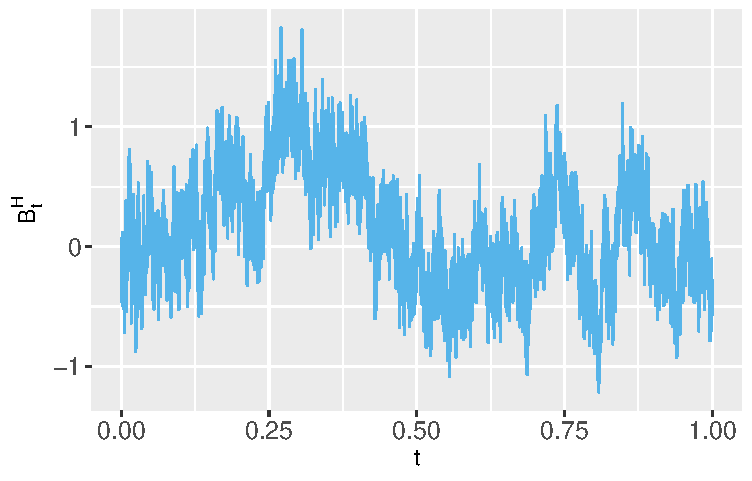
\includegraphics[scale=0.58]{fig/img/fBM paths/fBM1,H0.2.pdf}\hfill
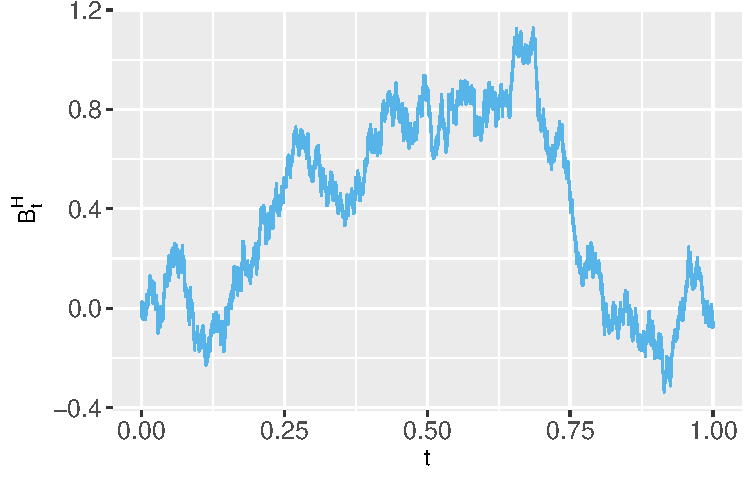
\includegraphics[scale=0.59]{fig/img/fBM paths/fBM2,H0.5.pdf}\hfill
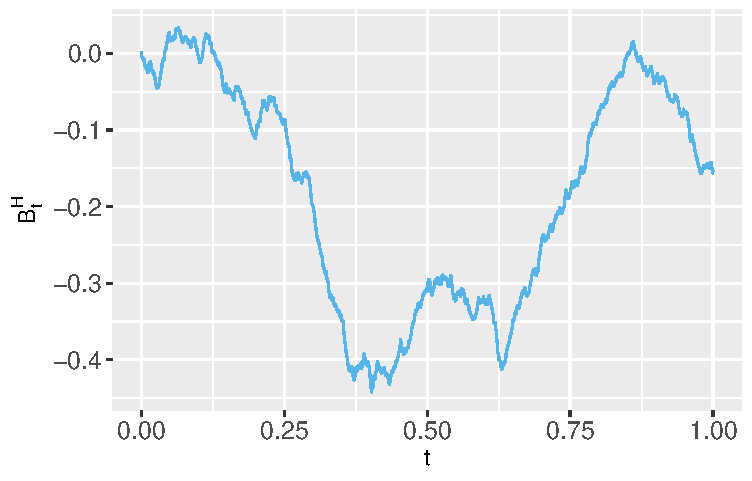
\includegraphics[scale=0.6]{fig/img/fBM paths/fBM3,H0.8.pdf}

\caption{Paths of fBMs of Hurst indices $0.2$ (top left), $0.5$ (top right), and $0.8$ (bottom).}
\label{fig:figure3}

\end{figure}
Figure \ref{fig:figure3} shows simulated fBM paths with $10,000$ points each. As was shown in Theorem \ref{existencethm}, the path of a fBM is almost surely Hölder continuous of order $\alpha\in(0,H)$ on compact intervals, and hence the Hurst index $H$ controls the roughness of the paths. In accordance with Figure \ref{fig:figure3}, the paths become less rough and more well-behaved as $H$ increases. However, for our purposes of modelling stochastic volatility, only the rough paths with $H<1/2$ will be of interest.
%Even though in theory, the eigenvalues \eqref{eigenvalues} are real, and the resulting vector $V$ is real by construction, one might still need to take the real part of these when implementing the method due to the nature of floating point arithmetic.
%The matrix $L$ can be computed more efficiently, if we utilize the fact that $\Gamma_N$ is Toeplitz matrix. 

\newpage
\textbf{Spørgsmål til vejledermøder:}
\begin{enumerate}
    \item \st{Hvorfor forskellige resultater ved de to simulationsprocedure?}
    \item \st{Skal jeg have beviset for eksistensen af fBM med?} 
    \item \st{Fatte selve formuleringen i projektforslaget} 
    \item \st{Volatility surface: "Overall shape does not change; At least to a first degree".}
    \item Kunne man ikke også kigge på at forecaste volatilitet med den nævnte OU-model? Og sammenligne med en anden model fx. GARCH eller lignende? 
    \item \st{Er "equal in law" og "equal in distribution" det samme?}
    \item "Nem måde" at web-scrape den seneste aktiekurs på fra yahoo?
    \item \st{Laese beviset for Proposition 2.14, da det er lidt hjemmebrygget}
    \item Kompleksiteten i circulant metoden
    \item Summationsindeks i beviset for Proposition 3.17.
\end{enumerate}
\textbf{Ting jeg skal huske}
\begin{enumerate}
    \item \st{Samme notation for autokovarians-funktionen for Gaussisk hvid stoej - Lige nu er der boede $\rho$ og $\gamma$.}
    \item \st{Samme notation for "equal in law" og "equal in distribution".}
    \item Autokovariansfunktioen defineret på naturlige tal, hele tal osv.?
    \item Styr pa kapitlet "Preliminary Theory"
\end{enumerate}